\documentclass{article}
\usepackage{../fasy-hw}
\usepackage{ wasysym }
\usepackage{graphicx}
\graphicspath{{./images/}}

%% UPDATE these variables:
\renewcommand{\hwnum}{1}
\title{Discrete Structures, Homework 1}
\author{Braeden Hunt (Tinnittin\#9115)}
\collab{n/a}
\date{due: 22 January 2021}

\begin{document}

\maketitle

This homework assignment should be
submitted as a single PDF file both to D2L and to Gradescope.

General homework expectations:
\begin{itemize}
    \item Homework should be typeset using LaTex.  (Note: if you are still
        having trouble with your setup, please reach out to the instructor and
        TA).
    \item Answers should be in complete sentences and proofread.
    \item You will not plagiarize.
    \item List collaborators at the start of each question using the
        \texttt{collab} command.
    \item Put your answers where the \texttt{todo} command currently is (and
        remove the \texttt{todo}, but not the word \texttt{Answer}).
\end{itemize}

% ============================================
% ============================================
\nextprob{Getting to Know Your Classmates}
\collab{n/a}
% ============================================
% ============================================

Find a different classmate for each of the following:
\begin{enumerate}
    \item Was born in the same month as you (year can be different).
        \paragraph{Answer} Mason Reyher and I were both born in September.

    \item Has a shared hobby with you.
        \paragraph{Answer} Duncan Platz and I both ski.

    \item Has the same middle initial as you.
        \paragraph{Answer} Robert Spyk and I both have middle names starting with the letter J.

    \item Lives in a different building than you.
        \paragraph{Answer} Ben Kiehn and I don't live in the same buidling.

    \item Has eaten at at least one restaurant or traveled to at least one city that you have not been
        (yet).
        \paragraph{Answer} Patrick O'Conner has been to Chicago, which I have not been to.

\end{enumerate}

% ============================================
% ============================================
\nextprob{Why Proofs?}
\collab{n/a}
% ============================================
% ============================================

Much of this class is spent learning how to prove things.  Explain why it is
important to you, as a computer scientist, to know how to prove things
mathematically.

\paragraph{Answer}

Proofs are very important to computer scientists, especialy when it comes to analyzing algorithms. In order to understand and evaluate different algorithms, we need to be able to prove that they work, how they work, how much resources they use, and how long they take to run. Also, proofs are based in the language of logic, and by learning/using proofs, you're applying logic. Computer science relies heavily on logical thinking and computation, so we are practicing those skills with proofs.


% ============================================
% ============================================
\nextprob{A Proof}
\collab{n/a}
% ============================================
% ============================================

Prove that $6\Z \subset 2\Z$.

\paragraph{Answer}

Let $n \in 6\Z.$ 

By definition of $6\Z$, we know that $n= 6*i$, where $i$ is an integer.

By factoring, we see that $n=2 * (3 * i)$.

Therefore, $n=2*k$, where $k=3*i$, which means that $n \in 2\Z$, as was to be shown.


% ============================================
% ============================================
\nextprob{Grace Hopper}
\collab{n/a}
% ============================================
% ============================================

Write a short (1-2 paragraph) biography of Grace Hopper.
\textbf{In your own words}, describe who they are and why they are important in
the history of computer science.  If you use external resources, please provide
proper citations.

\paragraph{Answer}

Grace Hopper was one of the founding "programmers" of computer science. Born in 1906, she was a pioneer in the computer science field. After receiving her masters and docorate in mathematics, worked on programming a computer at Harvard to help the U.S. Navy design ships. She worked extensively in developming computer languages, inventing the first complire and later the first human readable programming language. Her work in both the private and public sector greatly expanded the field of computer science and opened it up to many more people that just highly educated and trained mathematicians. A fun side note is that she was also the person who coined the term "bug" and "debug" in computer programs.

\parbox[t]{\linewidth}{\hangindent=7mm \noindent{“Grace Murray Hopper (1906-1992): A Legacy of Innovation and Service.” \textit{YaleNews}, 27 Feb. 2017, news.yale.edu/2017/02/10/grace-murray-hopper-1906-1992-legacy-innovation-and-service. }}

% ============================================
% ============================================
\nextprob{Bonus Question!}
\collab{\todo{}}
% ============================================
% ============================================

Use the `figure` environment to add a figure that provides the solution to
Exercises set 1.4, Problem 4.  Your figure can be hand drawn and scanned, or can
be made using a tool such as Inkscape.


\begin{figure}
\caption{Example Set 1.4 Problem 4}
\centering
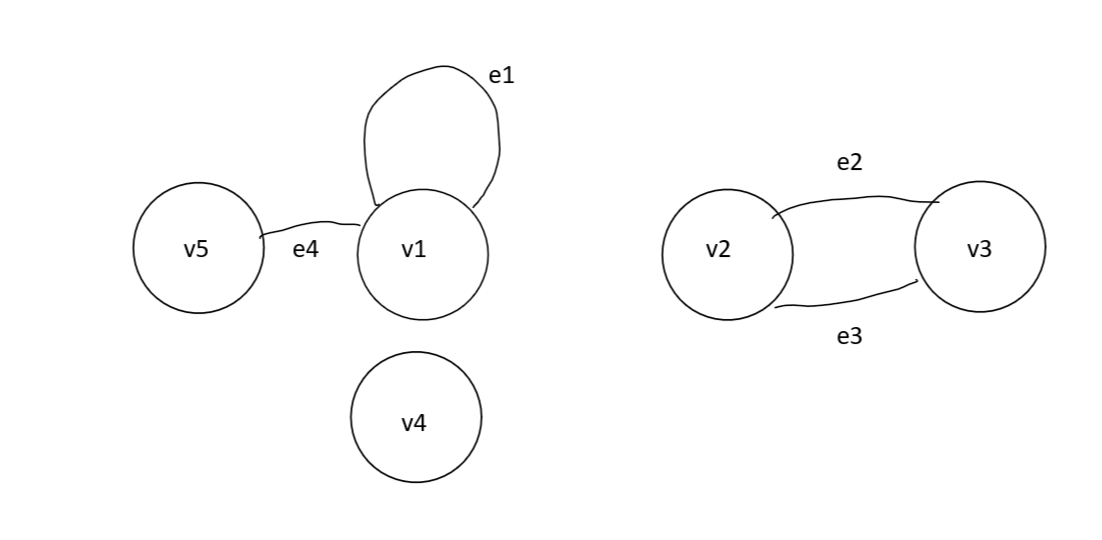
\includegraphics[width=0.5\textwidth]{figure}
\label{problem4}
\end{figure}
\paragraph{Answer} See Figure \ref{problem4}.
\end{document}

